\documentclass[../../main.tex]{subfiles}

\graphicspath{{../../fig/}}
\setcounter{section}{0}

\begin{document}
\chapter{Simons Observatory実験}
\section{Simons Observatory実験}
Simons Observatory実験 (以後、SOと呼ぶ) は、チリのアタカマ砂漠を拠点とする史上最大規模の地上CMB観測実験である。
現在、口径 $0.5\ \mathrm{m}$ の小口径望遠鏡 (Small Aperture Telescope, SAT) 3台と、
口径 $6\ \mathrm{m}$ の大口径望遠鏡 (Large Aperture Telescope, LAT) 1台を用いた観測が進められている。\cite{so:current_status}
検出器としてはTES (Transition Edge Sensor) 検出器を採用しており、SATにはそれぞれ約1万個ずつ、LATには約3万個の検出器が搭載されている。
合計約6万個もの検出器を通してCMBの変更を高精度で測定し、インフレーションに由来する原始重力波の検出や、
ニュートリノの有効世代数、ニュートリノ質量和の測定を目指す。\cite{so:science_forecast}

立体角 $\Omega$ 、開口面積 $A$、観測波長 $\lambda$ について、回折限界の関係式
\begin{equation}
    \Omega = \dfrac{\lambda^2}{A}
\end{equation}
を考えると、より大きな口径 $A$ を持つ望遠鏡ほどより高い角度分解能を有し、小角度の相関を観測するのに適していることがわかる。
その一方で、大口径の望遠鏡は一度に観測できる範囲も小さくなるため、大角度の相関を観測するのに時間を要し、大気揺らぎの影響を受けやすくなってしまう。
以上の理由から、小口径で大角度相関を調べるSATと、大口径で小角度相関を調べるLATを組み合わせることで、CMBのより精密な測定を実現する。

\section{Large Aperture Telescope (LAT)}
\section{Small Aperture Telescope (SAT)}
\subsection{TES検出器}

\subsection{極低温連続回転式半波長板 (HWP)}
大気による熱放射は常に揺らいでいる。
これは大気による $1/f$ ノイズとして知られ、CMB偏光観測実験においては、このノイズとCMB偏光信号を分離することが重要である。
Simons Observatoryでは、この大気による熱放射を取り除くために、極低温連続回転式半波長板(cryogenic continuously rotating Half-Wave Plate, 以後、単にCHWPと呼ぶ)を用いる。\cite{so:hwp_yamada}

一般に、HWPは複屈折の特性を持つ素材からなり、素子中のある決まった軸に対して電場成分を反転させる。
すなわち、HWPに入射する光の電場 $\bm{E}$ はHWPを通過することで
\begin{align}
    E_{1} &= E_{1} \\
    E_{2} &= -E_{2}
\end{align}
となる。ここで、$1, 2$ はそれぞれHWPの光学軸を表し、1軸に対して電場成分が反転している。
入射光として偏光角がHWPの1軸から測って $\chi$ であるような直線偏光した光を考える。
HWPを通過した後の偏光角は $-\chi$ となり、偏光が1軸対称に反転、つまり $-2\chi$ だけ変化する。(図\ref{fig:so-hwp_satoru})
この性質により、入力信号のストークスパラメータがそれぞれ $I_{\mathrm{in}}(t), Q_{\mathrm{in}}(t), U_{\mathrm{in}}(t)$ であるとき、出力信号 $d_m(t)$ は
\begin{equation}
    d_{\mathrm{m}}(t) = I_{\mathrm{in}}(t) + \varepsilon\Re\qty[\qty(Q_{\mathrm{in}}(t)+iU_{\mathrm{in}}(t))\exp(-i 4\chi)]
\end{equation}
となる。ここで、$\varepsilon$ は変調効率である。SOでは、HWPを $2\ \mathrm{Hz}$ で回転させることで、連続的に入射する直線偏光による信号を $8\ \mathrm{Hz}$ に変調して出力する。
HWPの角振動数を $\omega_{\mathrm{HWP}}$ とすると、$\chi = \omega_{\mathrm{HWP}}t$ と表され、出力信号は
\begin{equation}
    d_{\mathrm{m}}(t) = I_{\mathrm{in}}(t) + \varepsilon\Re\qty[\qty(Q_{\mathrm{in}}(t)+iU_{\mathrm{in}}(t))\exp(-i 4\omega_{\mathrm{HWP}}t)]
\end{equation}
となる。検出器はある偏光角方向 $\theta_{\mathrm{det}}$ にのみ感度を持つため、最終的に検出器が読み出す信号 $d_{\mathrm{m}, \mathrm{det}}$ は
\begin{equation}
    \label{eq:so-hwp_modulation}
    d_{\mathrm{m}, \mathrm{det}}(t) = I_{\mathrm{in}}(t) + \varepsilon\Re\qty[\qty(Q_{\mathrm{in}}(t)+iU_{\mathrm{in}}(t))\exp\qty{-i \qty(4\omega_{\mathrm{HWP}}t - 2\theta_{\mathrm{det}})}]
\end{equation}
となる。この信号のフーリエ変換は
\begin{equation}
    \begin{split}
        \tilde{d}_{\mathrm{m}, \mathrm{det}}(\Omega) = &\tilde{I}_{\mathrm{in}}(\Omega) \\
            &+ \dfrac{\varepsilon}{2}\qty[\qty{\tilde{Q}_{\mathrm{in}}(\Omega+4\omega_{\mathrm{HWP}})+i\tilde{U}_{\mathrm{in}}(\Omega+4\omega_{\mathrm{HWP}})}\exp\qty(i2\theta_{\mathrm{det}})] \\
            &+ \dfrac{\varepsilon}{2}\qty[\qty{\tilde{Q}_{\mathrm{in}}(\Omega-4\omega_{\mathrm{HWP}})-i\tilde{U}_{\mathrm{in}}(\Omega-4\omega_{\mathrm{HWP}})}\exp\qty(i2\theta_{\mathrm{det}})]
    \end{split}
\end{equation}
である。この式はほとんど時間変化しない信号$(\Omega\sim0)$がHWPを通過することで、周波数 $\pm 4\omega_{\mathrm{HWP}}$ のところに移ることを示している。
このようにして、元々 $1/f$ ノイズが大きかった低周波帯の信号を、ノイズの少ない高周波帯に変換できる。
$Q_{\mathrm{in}}+iU_{\mathrm{in}}$ を得るためには、$+4\omega_{\mathrm{HWP}}$ のまわりのみを通すバンドパスフィルタ $\mathcal{F}^{\mathrm{BPF}}$ を通した後、2倍して位相を元に戻せば良い。
つまり、復調後に得られる信号 $d_{\mathrm{d, det}}$ は
\begin{align}
    d_{\mathrm{d, det}}(t) &= \mathcal{F}^{\mathrm{BPF}}\qty[d_{\mathrm{m,det}}(t)]\times 2\exp\qty(i4\omega_{\mathrm{HWP}}t) \\
    &= \varepsilon\qty[Q_{\mathrm{in}}(t) + iU_{\mathrm{in}}(t)]\exp\qty[i2\theta_{\mathrm{det}}]
\end{align}
となっている。

\begin{figure}[H]
    \centering
    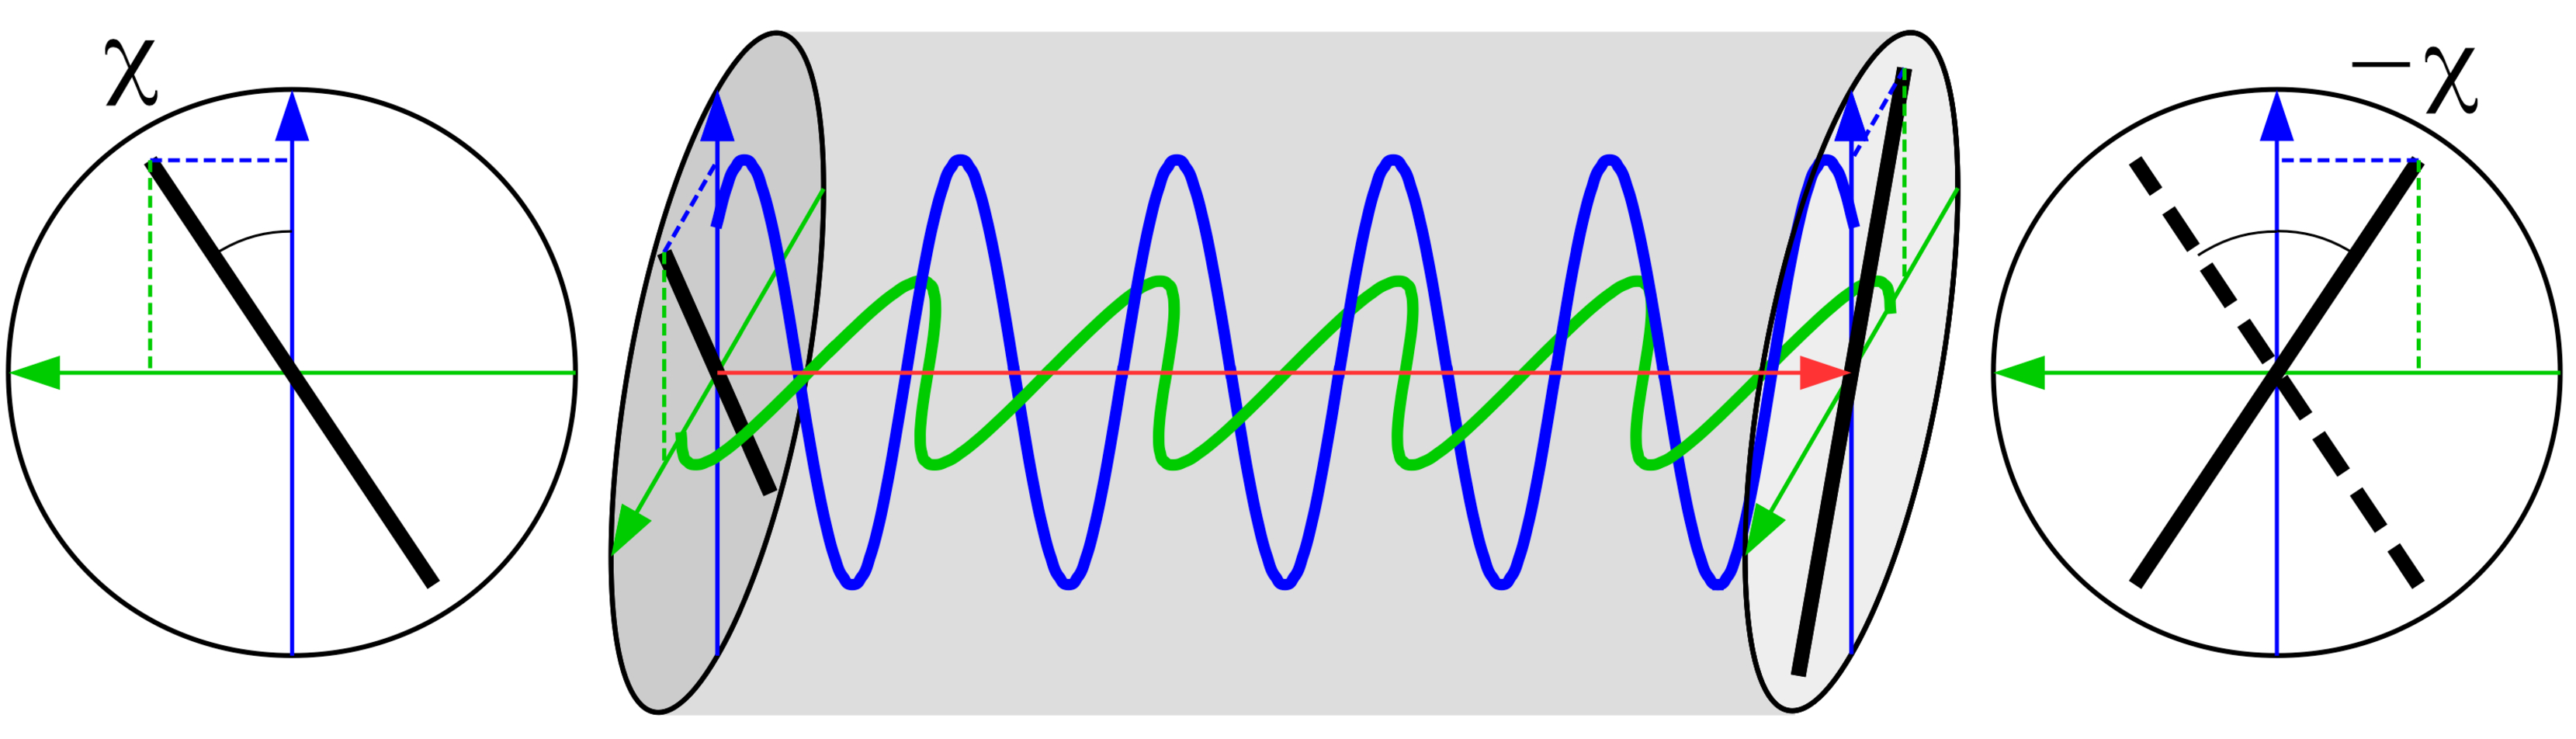
\includegraphics[width=0.8\textwidth]{simons_observatory/hwp_satoru.pdf}
    \caption{HWPを通過することで、偏光角が変化することを示した概念図。青い軸が1軸、緑の軸が2軸に対応する。
    入射した直線偏光の偏光角が1軸に対して $\chi$ であり、複屈折によって $-2\chi$ だけ変化する。}
    \label{fig:so-hwp_satoru}
\end{figure}


\end{document}